
\chapter{Fonctionnement de l'application}
Toutes les pièces du puzzle ont été introduit, il ne manque plus qu'a les assembler pour construire le chatbot. Comme expliqué ci-dessus, les algorithmes de prédictions seront tous dans l'api via le protocole REST, le chatbot sera équipé d'une brique NLU et CORE, un formulaire d'action qui va s'occuper de remplir les slots et appeler l'api de prédiction.\linebreak
Dans ce chapitre nous allons voir le bot en action.

Voici une interaction avec le chatbot:

\begin{description}
\item[user]: bonjour
\item[bot]: Bonjour je suis marie, quelle est votre soucie
\item[user]: voilà je vous appelle car ma chaudière est en panne
\item[bot]: Parler moi plus en détail de votre chaudière qui est en panne, si vous en avait
\item[user]: elle ne fonctionne plus quand je l'allume
\item[bot]: Je vais faire monter l'information au service concerné qui vous rappellera
\item[bot]: au revoir.	
\end{description}

Le chatbot possède aussi un port serveur, les appelles se font via le protocole REST entièrement en \textit{POST}.\linebreak
Le premier souci du chatbot c'est que nous ne pouvons pas faire passer à travers le chatbot une interaction entre deux clients sans que celui-ci ne consomme les données, donc il a fallu un programme fessant office de routeur pour les conversations de l'utilisateur, soit le schéma suivant:

\begin{center}
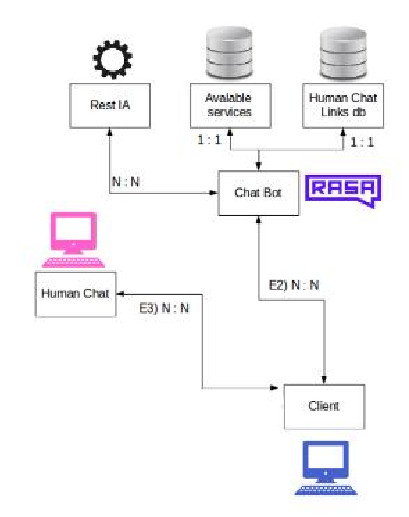
\includegraphics[scale=0.9]{img/plans.jpg}
\end{center}

Lors de la phase de développement du projet, le programme routeur était un programme python, qui attendait un certain paquet provenant du bot pour pouvoir changer l'url d’envois des données vers un service client. Une fonctionnalité en plus est que le bot à un annuaire (noté par la base de données \textit{Human Chat Links db} qui redirige le client vers tel endpoint de telle adresse de tel service.\linebreak

\section{Implémentations futures}

Dans ce qu'il reste du projet, nous devons brancher le chatbot sur une interface pouvant être compatible avec un téléphone, pour le travail en cours, nous avons choisis une solution nommé \textit{Softphone} qui va simuler un vrai téléphone mais en logiciel. La sortie de celui-ci sera redirigé dans le programme et l'entrée du softphone est réglé sur auto commutateur téléphonique nommé \textit{Asterisk}, il va lui s'occuper de la liaison entre les vrai téléphone et le softphone.

Nous devons avoir une brique transformant la voix en texte et inversement, nous allons utiliser \textit{DeepSpeech} la librairie de Mozilla qui va nous permettre via des algorithmes Tensorflow et Seq2Seq de générer un modèle répondant à nos besoins.\linebreak

\chapter{Conclusion}

Ce fut un stage riche en découverte, une bonne continuation des cours de machines learning proposé à la faculté, un branchement plus que parfait. Lorsque qu'à la fac nous apprenons les bases du machine learning, de la fouille de données, et quelques implémentations avec des datasets plus orienté numérique, le stage s'est directement enchaîné avec du travail sur le langage naturelle.\linebreak
la méthodologie agile m'as permis de me donner des objectifs à réaliser dans des délai autre que la deadline du projet.\linebreak
J'ai gagné en compétence dans l'art de la fouille de données et dans l'analyse de données en ayant travaillé avec des donnée clients car qui a donné un vrai terrain d'apprentissage du métier de \textit{Data Analyste} dans la vie professionnel.
